% !TEX encoding = UTF-8 Unicode
% -*- coding: UTF-8; -*-
% vim: set fenc=utf-8

\chapter{Trabalhos Relacionados}%
\label{chap:trabalhos-relacionados}

Dado que o principal objetivo dessa monografia é a apresentação de um processador de consultas integrado à arquitetura ARMFUL que será abordada no \autoref{chap:arquitetura-armful}, nesse capítulo serão abordados alguns trabalhos e algumas publicações relacionados a ela, no que diz respeito a simulações científicas, a \textit{workflows} científicos, a proveniência de dados e, em especial, a \textbf{tipos de consulta} que podem ser realizados.

\section{Tipos de consulta}%
\label{sec:tipos-de-consulta}

Conforme introduzimos na \autoref{sec:motivacao}, existem três tipos básicos de consultas que podem ser realizados em uma base de dados de proveniência de uma simulação computacional~\cite{silva2015analyzing,silva2015propostadoutorado}:

\begin{enumerate}
    \item análise de dados científicos isolados de um único arquivo, envolvendo a extração de conteúdos específicos de domínio, que será abordado na \autoref{sec:analise-de-dados-cientificos-isolados};
    \item rastreio de fluxos de múltiplos arquivos relacionados através de transformações de dados correspondentes, discutido na \autoref{sec:rastreio-de-fluxos-de-arquivos}; e
    \item rastreio de elementos de dados relacionados em múltiplos arquivos, que será elucidado na \autoref{sec:rastreio-de-elemento-de-dados-em-multiplos-arquivos}.
\end{enumerate}

Consultas do tipo 1 requerem apenas acesso a um único arquivo, enquanto consultas dos tipos 2 e 3 necessitam do apoio de fluxo de dados da simulação computacional~\cite{silva2015analyzing}.

\perrotta{REVIEW: tudo bem colocar esse exemplo aqui, ou é melhor incluí-lo no final?}

\subsection{Um exemplo}

A \autoref{fig:types-of-queries-1-2-3} apresenta um exemplo que envolve os três tipos de consulta citados na \autoref{sec:tipos-de-consulta}:

\begin{itemize}
    \item exemplo de consulta do tipo 1: usuário realiza uma consulta específica do domínio ao conteúdo do arquivo \mbox{\texttt{projected{\_}images.tbl}}. Os atributos FA e FB (marcados com linhas vermelhas) são acessados e capturados para a subsequente análise de transformações lineares realizadas pelo programa de projeção presente na simulação computacional com uma configuração pré-definida;
    \item exemplo de consulta do tipo 2: as setas de cor preta representam a sequência do fluxo de arquivos nos formatos \texttt{TBL} e \texttt{FITS}, os quais são projetados em outros arquivos \texttt{TBL} e depois transformados para eventualmente criar um arquivo de imagem no formato JPG (\mbox{\texttt{mosaic.jpg}}). O registro desses relacionamentos permite a possibilidade do rastreio dos arquivos intermediários que geram o arquivo de imagem.
    \item exemplo de consulta do tipo 3: podemos visualizar um dos fluxos de elementos de dados através da representação das setas na cor vermelha. Nesse exemplo, o atributo CRVAL1 é utilizado como chave para relacionar os dados científicos em diferentes arquivos. Dessa forma, através desse atributo, o arquivo \mbox{\texttt{hdu{\_}1n.fits}} pode ser relacionado ao elemento de dados FB cujo valor é 0.001969140 do arquivo \mbox{\texttt{projected{\_}images.tbl}}.
\end{itemize}

\begin{figure}[htb]
    \centering
    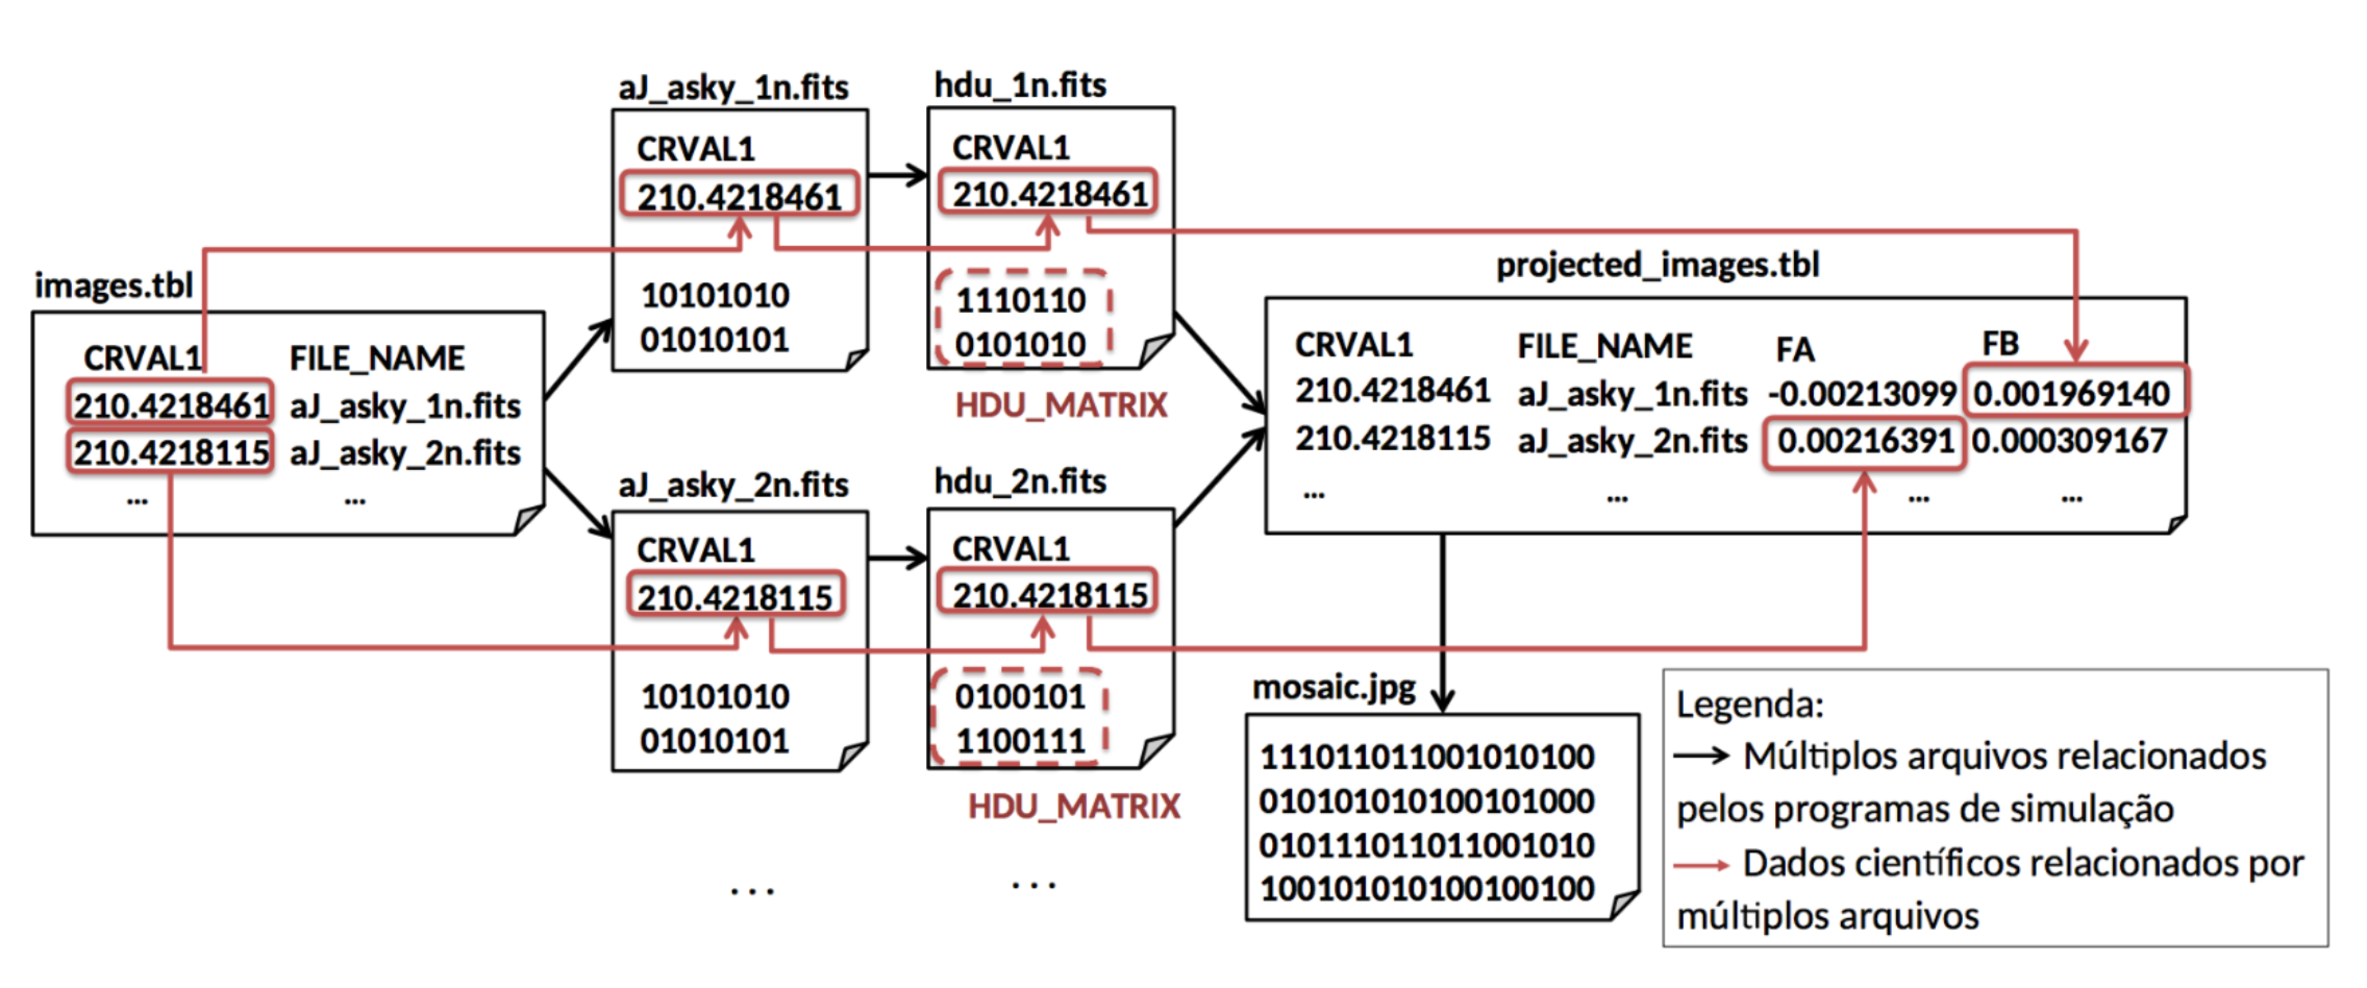
\includegraphics[width=\textwidth]{img/types-of-queries-1-2-3}
    \caption[Exemplo de análise de uma simulação de astronomia]{Exemplo de uma simulação de astronomia para análise de arquivos de dados científicos. Encontrada originalmente em~\cite{silva2015propostadoutorado}.}%
    \label{fig:types-of-queries-1-2-3}
\end{figure}

\section{Análise de dados científicos isolados}%
\label{sec:analise-de-dados-cientificos-isolados}

Consultas do \textbf{tipo 1} são caracterizadas pela \textbf{análise} (do inglês: \textit{parsing}) \textbf{de dados científicos}, encontrados em arquivos que foram produtos de uma simulação computacional, e envolve tipicamente a \textbf{extração} ou \textbf{interpretação} desses dados de acordo com o domínio da aplicação da simulação. É necessário conhecer a estruturação e~/~ou a codificação utilizada nesses arquivos para que seja possível acessá-los e extrair um significado semântico dos dados do mesmo; além disso, cada formato de arquivo possui programas específicos e peculiares para a sua análise e extração: por exemplo, um arquivo em formato de imagem tal como o \abbrev{PNG}{\textit{Portable Network Graphics}} PNG (Portable Network Graphics) pode ser analisado (visualizado) por um editor de imagens, enquanto que um arquivo em formato de música tal como o \abbrev{WAV}{Waveform Audio File Format} WAV (\textit{Waveform Audio File Format}) pode ser analisado (reproduzido) por um \textit{player} de áudio. Em particular, destaca-se que a semântica da análise --- reprodução, visualização, extração, etc --- é inerente ao tipo de arquivo analisado.

Esses dados e seus respectivos arquivos podem estar ou não em formato binário; por exemplo, um arquivo em formato \abbrev{JSON}{JavaScript Object Notation} JSON (JavaScript Object Notation) geralmente contém dados em formato de texto; enquanto que um arquivo FITS (Flexible Image Transport System)~\cite{greisen2002representations}, utilizado em astronomia, pode possuir parte de seus dados em formato binário assim como o NetCDF (Network Common Data Form)~\cite{rew1990netcdf}, utilizado em dinâmica de fluidos computacionais, e o HDF5~\cite{folk1999hdf5}, utilizado em várias aplicações distintas.

Consultas do tipo 1 são as mais simples de serem realizadas em relação às outras, pois elas são auto-contidas no que diz respeito aos dados científicos, isto é, apenas a presença desses dados é suficiente para que esse tipo de consulta possa ser realizado: não é necessária a especificação sobre o fluxo de dados da simulação computacional.

\perrotta{REVIEW: Extratores?? Como obtive os dados?}

\section{Rastreio de fluxos de arquivos}%
\label{sec:rastreio-de-fluxos-de-arquivos}

Consultas do \textbf{tipo 2} são caracterizadas pelo rastreio do \textbf{fluxo de arquivos}, que se relacionam através de transformações de dados. Elas são frequentemente apoiadas por sistemas de \textit{workflows} científicos, tais como o Chiron~\cite{ogasawara2011algebraic}, o Pegasus~\cite{deelman2005pegasus} e o Kepler~\cite{ludascher2006scientific}. Através desse tipo de consulta, que busca informações de proveniência retrospectiva, os usuários são capazes de rastrear, em uma míriade de arquivos de uma simulação computacional em larga escala, qual foi o fluxo de arquivos que gerou determinados conjuntos de dados finais a partir de quais conjutos de dados iniciais.

Um exemplo de ferramenta que é capaz de realizar consultas do tipo 2 é o \textit{NoWorkflow}~\cite{murta2014noworkflow} (do inglês: \textit{\textbf{n}ot \textbf{o}nly \textbf{workflow}}), que captura de forma transparente a proveniência de \textit{scripts} escritos na linguagem de programação Python. Essa captura é feita a nível de funções (subtorinas) da linguagem e, em particular, chamadas de sistema do tipo \emph{open} (=leitura de arquivos) presentes nos \textit{scripts} são capturadas, assim como os arquivos que lhe são passados como argumentos, que então são armazenados em um banco de dados relacional que identifica as relações (de entrada e de saída) entre esses arquivos. Dessa maneira, o \textit{NoWorkflow} possui toda a informação de proveniência retrospectiva~\cite{Pimentel2016} necessária para consultar o fluxo dos arquivos lidos e escritos durante a execução dos \textit{scripts}\footnote{Nesse contexto, um \textit{script} é análogo a um conjunto de transformações de dados, representando um programa científico.}.

Outra ferramenta que suporta consultas do tipo 2 é o \textit{YesWorkflow}~\cite{mcphillips2015yesworkflow}, que permite que os usuários façam anotações na forma de comentários especiais em seus \textit{scripts} e subsequentemente extrai e analisa esses comentários, representando os \textit{scripts} na forma de entidades e relações entre elas, formando e definindo um fluxo de dados. O \textit{YesWorkflow} pode ser utilizado em qualquer \textit{script}, não se limitando somente a Python, diferentemente do \textit{NoWorkflow}; mas, em contrapartida, ele requer anotações explícitas da parte do usuário, não sendo capaz de extrair informações de proveniência automaticamente como o \textit{NoWorkflow}~\cite{Pimentel2016}. Os comentários etiquetam regiões arbitrárias dos \textit{scripts}, associando valores a elas, os quais podem correlacionar e fazer associações a outras regiões; desse modo, um conjunto de comentários é capaz de especificar o fluxo de arquivos do fluxo de dados.

Citamos mais um exemplo de ferramenta que é capaz de realizar consultas do tipo 2, o Tigres~\cite{hendrix2016tigres}, que é inspirado no paradigma \textit{MapReduce} e suporta a criação de fluxos de dados sequenciais e paralelos. O Tigres é utilizado através de uma \abbrev{API}{Application Programming Interface} API (do inglês, Application Programming Interface) de \textit{templates} escrita em Python, com a qual o usuário define elementos do fluxo de dados e monitora a execução de programas científicos. Esses \textit{templates} funcionam como blocos de construção, que executam tarefas sequencialmente e geram informações de dependência e de proveniência entre os mesmos, tanto a nível prospectivo quanto a nível retrospectivo.

\section{Rastreio de fluxo de elementos de dados em múltiplos arquivos}%
\label{sec:rastreio-de-elemento-de-dados-em-multiplos-arquivos}

Consultas do \textbf{tipo 3} envolvem o rastreio de \textbf{elementos de dados relacionados} em \textbf{múltiplos arquivos}. Nesse sentido, são uma extensão das consultas do tipo 2, uma vez que é necessária uma granularidade mais fina para o fluxo, no nível de elementos de dados, e não apenas no nível do fluxo de arquivos.

O estado da arte no que diz respeito a soluções para análises de dados científicos em simulações científicas concentra-se hoje no apoio a consultas do tipo 1~\cite{alagiannis2012nodb,karpathiotakis2014adaptive,wu2009fastbit,folk1999hdf5,silva2015propostadoutorado} e do tipo 2~\cite{murta2014noworkflow,mcphillips2015yesworkflow,hendrix2016tigres,Pimentel2016}, como vimos em alguns exemplos nas seções anteriores. No entanto, algumas soluções para consultas do tipo 3 foram apresentadas nos últimos anos e vêm se consolidando recentemente.

Por exemplo, o \textit{NoWorkflow}, mencionado na \autoref{sec:rastreio-de-fluxos-de-arquivos}, também possui suporte a consultas do tipo 3, permitindo o rastreio de elementos de dados em nível de variáveis, de funções e de classes em \textit{scripts}, porém ele se limita somente a \textit{scripts} escritos na linguagem Python~\cite{murta2014noworkflow}

Outro paradigma que suporta consultas do tipo 3 é o da arquitetura ARMFUL, que é baseada em componentes e é instanciada, por exemplo, como o \textit{DfAnalyzer} em~\cite{silva2017raw}. Eles serão abordados detalhadamente no \autoref{chap:arquitetura-armful}.

\perrotta{REVIEW: DfAnalyzer (grupo) -- o que mais falar aqui?, CCPE (mais sistemas) - não entendi o que seria isso. Como expandir essa seção?}